\subsection{Python}

Covering some very useful cases of Python code for development. Based on books by Allen \cite{downey_2016}, Luciano \cite{ramalho_2016}, and...

\subsubsection{Directory and Files}

To work with files and directory, use the following snippet of code to get current path:
\begin{lstlisting}[language=Python]
import os
cwd = os.getcwd()
\end{lstlisting}
To find absolute path of file:
\begin{lstlisting}[language=Python]
filepath = os.path.abspath('file.txt')
\end{lstlisting}
To get parent folder of current file:
\begin{lstlisting}[language=Python]
parentfolder = os.path.dirname(cwd)
\end{lstlisting}
To check if file or directory exists:
\begin{lstlisting}[language=Python]
os.path.exists('file.txt')
\end{lstlisting}
To check if following is a directory, or is a file
\begin{lstlisting}[language=Python]
os.path.isdir('/dir/subdir')
os.path.isfile('file.txt')
\end{lstlisting}
To get list of files in given directory
\begin{lstlisting}[language=Python]
os.listdir(cwd)
\end{lstlisting}

For modules, the files should have the following code:
\begin{lstlisting}[language=Python]
if __name__ == '__main__':
	print(func(var1)) # Do something
\end{lstlisting}
If this code is ran as script, then '\_\_main\_\_' will run; if code is imported as module, then this is skipped.

\subsubsection{Python Data Model}

Special methods are methods that are meant to be called by the Python interpreter, and is usually implicit. To invoke a special method, call the related builtin function (e.g., len, iter, str, etc.). These are faster than method calls. The methods can be emulated in classes as follows:
\begin{enumerate}[label=\roman*.]
\setlength{\itemsep}{0pt}
\item Numeric Types: corresponding to operators such as $+$. An example in Euclidean space
\begin{lstlisting}[language=Python]
def __abs__(self):
	return math.hypot(self.x, self.y)
	
def __add__(self, value):
	return Object(self.x + value.x, self.y + value.y)

def __mul__(self, scalar):
	return Object(self.x * scalar, self.y * scalar)
\end{lstlisting}
\item String Representation: f-string gets standard representations of attributes to be displayed, which can then be used with the print function
\begin{lstlisting}[language=Python]
def __repr__(self):
	return f'Object({self.x}, {self.y})'
\end{lstlisting}
\item Boolean Type: for calling the object in a Boolean context
\begin{lstlisting}[language=Python]
def __bool__(self):
	return bool(self.x or self.y)
\end{lstlisting}
\end{enumerate}

The overview of special methods in Python is as follows:
\begin{figure}[H]
\centering
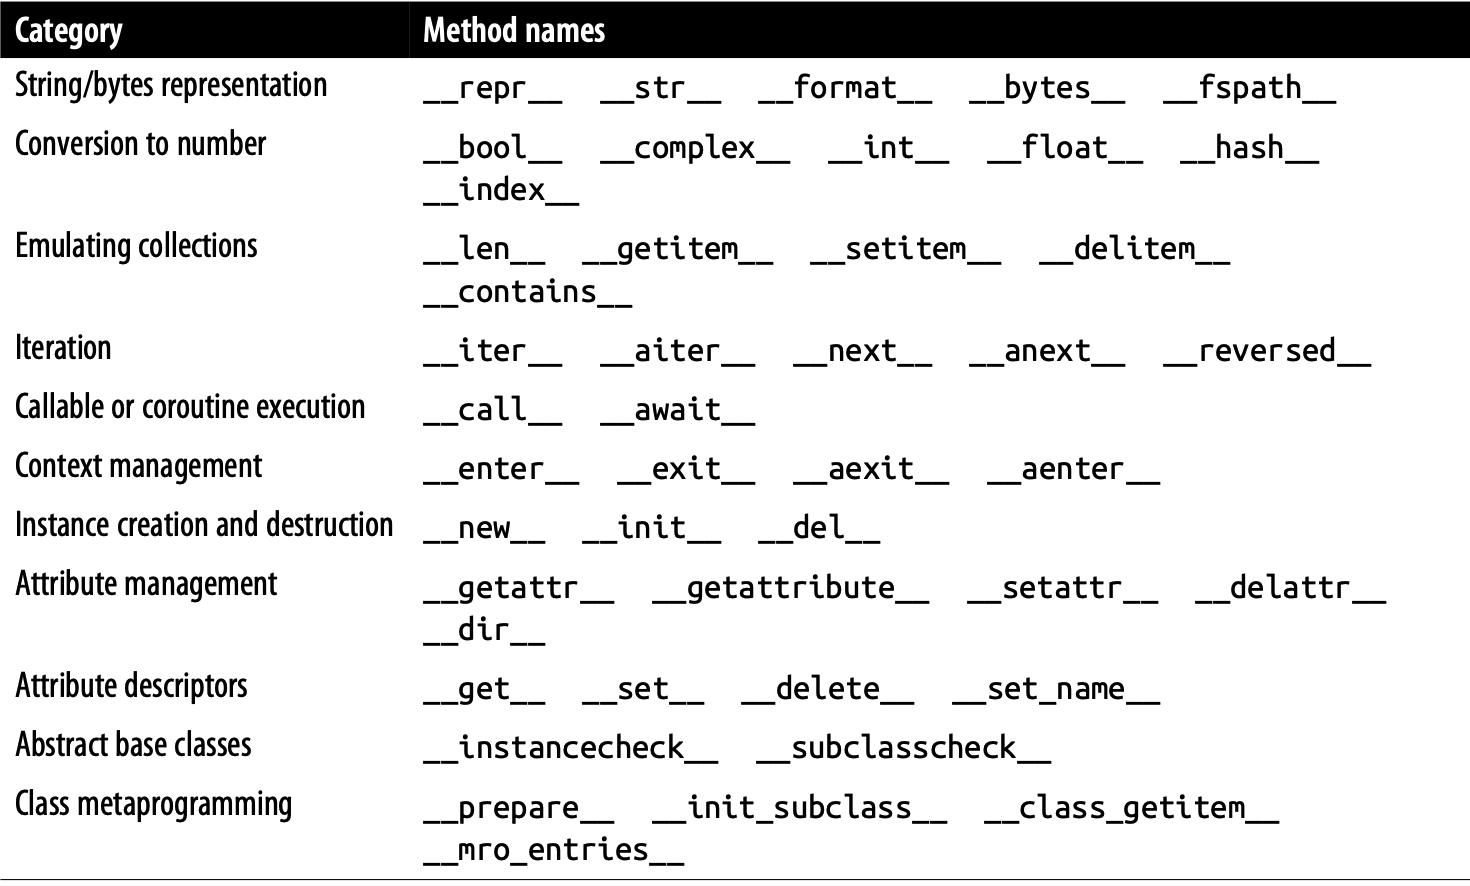
\includegraphics[scale=0.5]{appendix/python/specialmethods}
\caption{Special methods in Python}
\end{figure}